\chapter{Results}\label{results}
	This chapter discusses the performance as well as the limits of the proposed algorithms. 
	
		\section{BubbleProfiles}\label{result_profiles}
			
			\subsubsection{Performance}
			After training for 14 epochs, the testing accuracy converged to 96.8\%, which is a very good result for a binary classifier. 

			For validation, 20 more manually annotated small images were used, each containing from 10 to 20 bubbles. Figure \ref{fig:bubbleNet_result} illustrates the performance of algorithm \ref{algo:bubbleNet}.  
			The algorithm achieved mAP@.5IoU = 91.5\% and mAP@.3IoU = 93\%. Note that this is slightly worse than the classification accuracy result. This is due to the occasionally unprecise radius computation, which gets penalized by the mAP@p-IoU criterion. 
			
			In figure \ref{bubb_dist_1}, algorithm \ref{algo:bubbleNet} was applied to an image from the validation data set to produce a bubble distribution. Since the bubble radii were determined with a subpixel accuracy, bubble distributions are represented as a histogram with a bin size of $9 \, \mu m$. It can be observed that most bubbles have a size between $300 \, \mu m$ and $480 \mu m$. According to the technical specifications of the bubble generator, bubble radii between $100 \, \mu m$ and $400 \, \mu$ are expected. Images were captured at a distance of about $50 \, cm$ from the bubble generator $5.7 \, cm$ beneath the water surface. This leaves enough time for bubbles to merge and become larger. Thus, it can be concluded that the bubble distribution is roughly in agreement with the expected distribution given by the manufacturer of bubble generator.
			
			\subsubsection{Limits}
			The bubble radius is determined by computing the distance between the bright, lower peak and the dim, upper peak. Therefore, the smallest detectable bubble depends on how well the two peaks can be distinguished from each other.
			 This in turn depends on the smoothing filter applied to the vertical profile signal before peak extraction. A Gaussian smoothing filter with $\sigma = 4 \, px$ was used for both algorithms. This effectively sets the limit for the smallest detectable radius to $5 \, px$, i.e.\ $110 \, \mu m$ after calibration. The largest detectable bubble has a radius of $50 \, px$ as already discussed in section \ref{signal_extraction}. 
			 
			 The smallest detectable bubble radius can be further improved by increasing the magnification factor, as long as the assumptions discussed in section \ref{bubble_physics} are met, i.e.\ diffraction and Mie scattering are negligible. 
			 
			 
			
			\begin{figure}
				\centering
				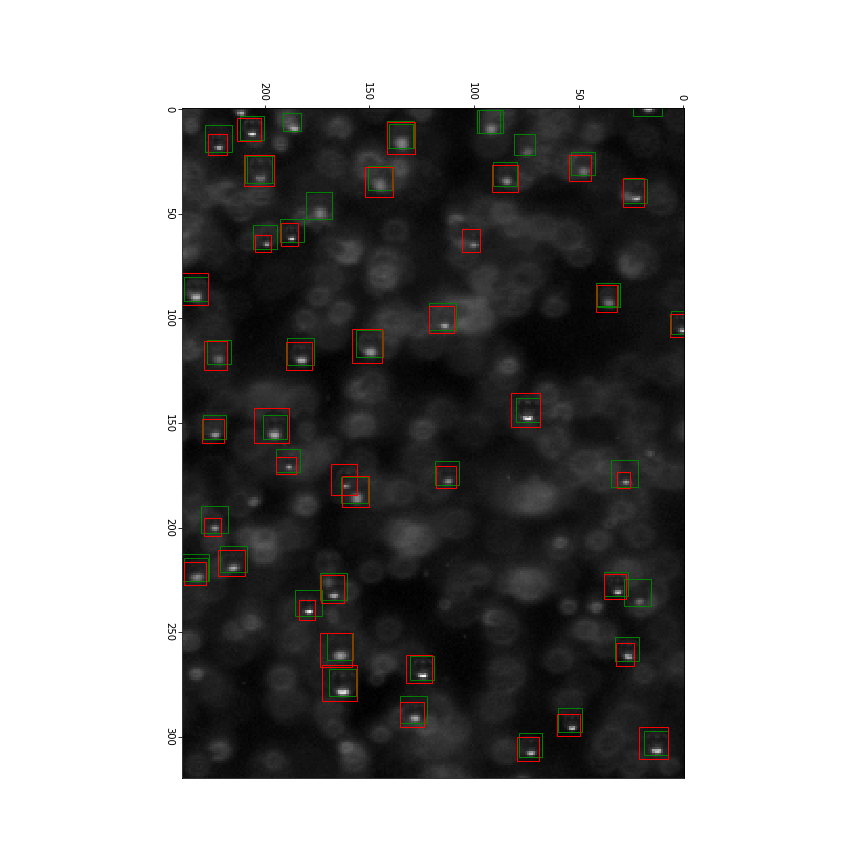
\includegraphics[scale=0.8]{images/bubbleNet_validation_result.png}
				\caption{Validation of algorithm \ref{algo:bubbleNet}. Red: ground truth, green: predicted. Note how in this image, ground truth annotation was not done perfectly, so IoU results were likely slightly underestimated.}
				\label{fig:bubbleNet_result}
			\end{figure}


				\begin{figure}
					\begin{subfigure}[t]{.4\textwidth}
						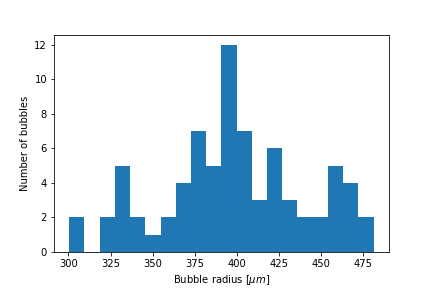
\includegraphics[scale=0.6]{graphs/b_val_0.png}
						\caption{Bubble distribution}
						\label{subfig:b_val_0}
					\end{subfigure}\hfill
					\begin{subfigure}[t]{.4\textwidth}
						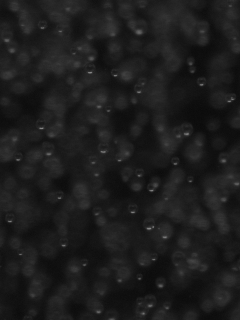
\includegraphics[scale=0.6]{images/val_1.png}
						\caption{Validation image}
						\label{subfig:val_0}
					\end{subfigure}
					\caption{Applying algorithm \ref{algo:bubbleNet} to a validation image captured with the aquarium setup. Image taken with the aquarium setup at 4\,cm below the water surface. Bubble radius has been calibrated with equation \ref{eq:radius_calib}, and measurement volume was limited to $6.6\, mm \times 9.6 \, mm \times 1\, cm$}
					\label{bubb_dist_1}
				\end{figure}




			\section{BubbleCurves}\label{result_curves}
			
				\subsubsection{Performance}
				This algorithm was only tested on the aquarium setup, since high bubble concentrations were not observed at the Aeolotron setup. 
				
				Using a validation set of 30 small images, each containing 30 to 40 bubbles, this algorithm achieved mAP@.5IoU = 89.3\%, which is slightly worse than algorithm \ref{algo:bubbleNet}. This is in part due to the high rate of overlap between bubbles, making curvature extraction less precise. 
				Nevertheless, the algorithm is reliable enough to be usable for bubble detection in high concentration images.					
				
				\subsubsection{Limits}
				Algorithm \ref{algo:bubbleCurves} relies on orientation to perform classification as well as to compute the bubble radius. Therefore, the smallest detectable bubble needs to show different orientations at different parts of the bubble. For instance, the orientation at the lower edge of the bubble needs to be different from the orientation at the side edge. Applying algorithm \ref{algo:bubbleCurves} to simulated data shows that the smallest detectable bubble radius is $5 \, px$, which corresponds to $160 \mu m$ after calibration. 
				The smallest detectable radius can also be improved by increasing the magnification. 
				
				
				
				
				
				
				
				
				
				
				